\begin{figure}
    \centering
    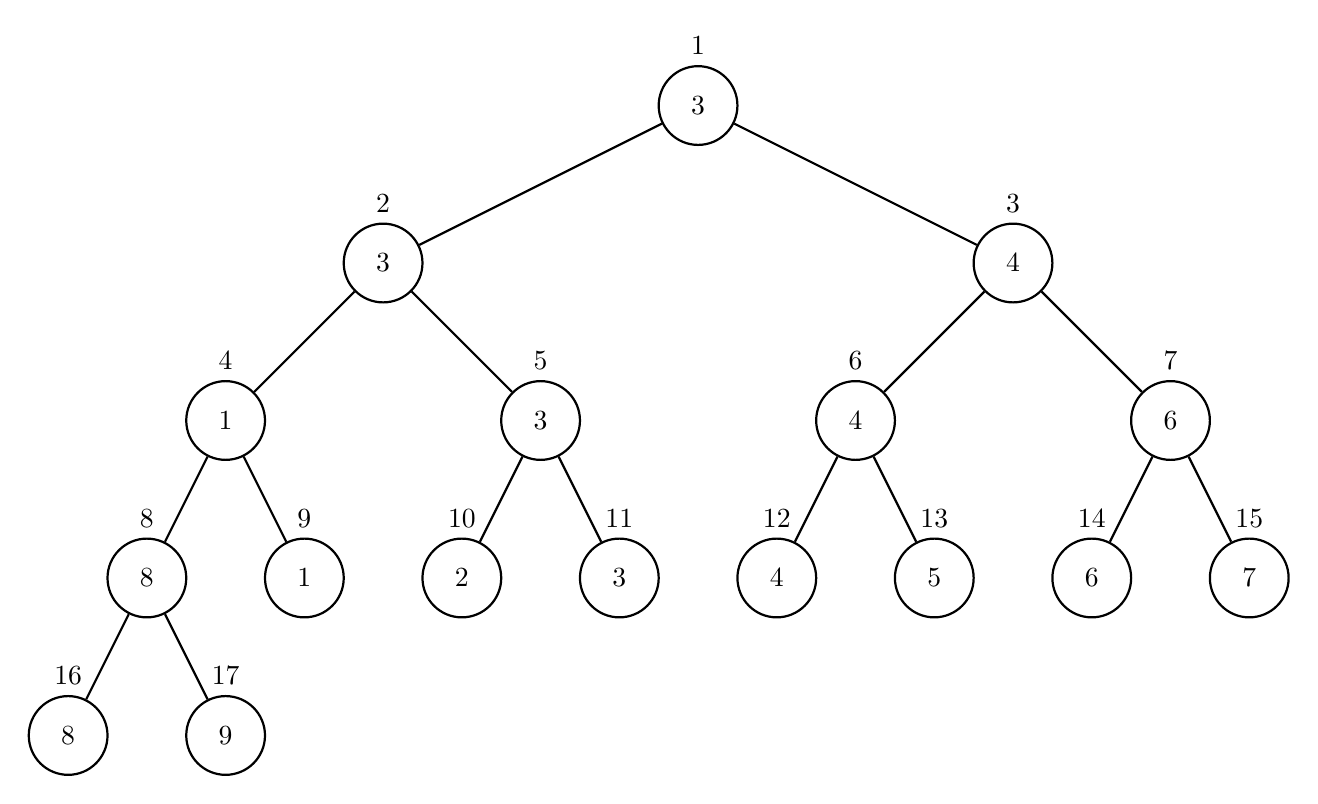
\begin{tikzpicture}[thick]
        \node[label={1},circle,draw,minimum size=1cm]
            (1) at (0,0) {$3$};
        \node[label={2},circle,draw,minimum size=1cm]
            (2) at (-4,-2) {$3$};
        \node[label={3},circle,draw,minimum size=1cm]
            (3) at (4,-2) {$4$};
        \node[label={4},circle,draw,minimum size=1cm]
            (4) at (-6,-4) {$1$};
        \node[label={5},circle,draw,minimum size=1cm]
            (5) at (-2,-4) {$3$};
        \node[label={6},circle,draw,minimum size=1cm]
            (6) at (2,-4) {$4$};
        \node[label={7},circle,draw,minimum size=1cm]
            (7) at (6,-4) {$6$};
        \node[label={8},circle,draw,minimum size=1cm]
            (8) at (-7,-6) {$8$};
        \node[label={9},circle,draw,minimum size=1cm]
            (9) at (-5,-6) {$1$};
        \node[label={10},circle,draw,minimum size=1cm]
            (10) at (-3,-6) {$2$};
        \node[label={11},circle,draw,minimum size=1cm]
            (11) at (-1,-6) {$3$};
        \node[label={12},circle,draw,minimum size=1cm]
            (12) at (1,-6) {$4$};
        \node[label={13},circle,draw,minimum size=1cm]
            (13) at (3,-6) {$5$};
        \node[label={14},circle,draw,minimum size=1cm]
            (14) at (5,-6) {$6$};
        \node[label={15},circle,draw,minimum size=1cm]
            (15) at (7,-6) {$7$};
        \node[label={16},circle,draw,minimum size=1cm]
            (16) at (-8,-8) {$8$};
        \node[label={17},circle,draw,minimum size=1cm]
            (17) at (-6,-8) {$9$};

        \draw[thick] (1) -- (2);
        \draw[thick] (2) -- (4);
        \draw[thick] (4) -- (8);
        \draw[thick] (4) -- (9);
        \draw[thick] (8) -- (16);
        \draw[thick] (8) -- (17);
        \draw[thick] (2) -- (5);
        \draw[thick] (5) -- (10);
        \draw[thick] (5) -- (11);
        \draw[thick] (1) -- (3);
        \draw[thick] (3) -- (6);
        \draw[thick] (3) -- (7);
        \draw[thick] (6) -- (12);
        \draw[thick] (6) -- (13);
        \draw[thick] (7) -- (14);
        \draw[thick] (7) -- (15);
    \end{tikzpicture}
    \caption[Representação da estrutura torneio]{Torneio com $9$
    elementos em que $3$ é o elemento com valor máximo.}
    \label{fig:torneio:exemplo}
\end{figure}